\chapter{Optical Density Measurement Techniques}
\label{chapter: LiteratureReview}

\par Several techniques have been developed which use light refraction as a principle to visualize changes in density. These methods can be grouped into classical techniques such as Shadowgraphy, Schlieren, Interferometry and modern methods, such as Background Oriented Schlieren and its variants. This section will provide a brief historical background on classical density gradient measurement techniques and explain how these methods have developed leading up to BOS. Then, a more detailed literature review is given in BOS and SBOS to better define the state of the art of these methods and provide context to the research gap that this thesis aims to fulfill.

%detailed description of the schlieren-based methods is given, finishing with laser %speckled BOS and the research gap.

\section{Classical Methods}

\par The earliest report of a density gradient measurement technique dates back to the 1600s, when Hooke tried to visualize the flow around a candle flame with the aid of a lens \cite{Settles2001}. His experiments resemble setups used for Shadowgraphy, where a test subject is positioned in between an observer and a light source, as shown in 
Figure \ref{fig: Hooke shadowgraphy}. The variations in the refractive index at the test section bends the light coming from the source, producing shadows and brighter regions captured by the observer. Shadowgraphy is valued by its simplicity, however it provides only qualitative results, as quantitative reconstruction is difficult due to second-derivative sensitivity on the line-of-sight integration. Nevertheless, Shadowgraphy continues to be an important flow visualization technique, complementing other more complex methods in the study of compressible flows \cite{Settles2017}.

\begin{figure}[htbp]
    \centering
    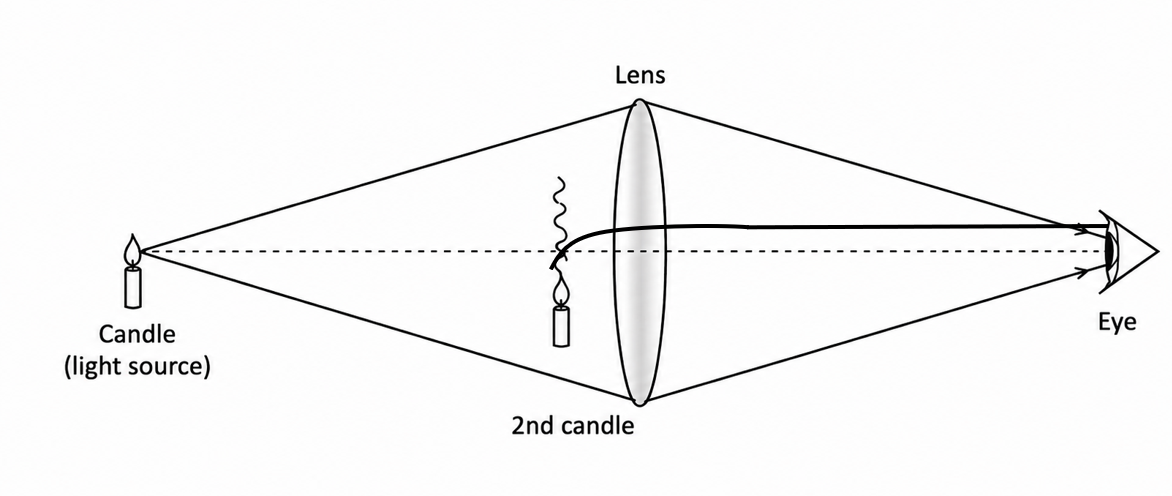
\includegraphics[width=0.8\textwidth]{figures/Hooke shadowgraphy setup.png}
    \caption{Hooke’s shadowgraphy setup, credit Settles \cite{Settles2001}}
    \label{fig: Hooke shadowgraphy}
\end{figure}

\par In the 19th century, Toepler coined the term “Schlieren” and was the first to apply the technique as a scientific tool \cite{Settles2001}. Toepler’s setup used a lens to focus the distorted light coming from the test section to a point where a knife’s edge was placed to block half of the image. The knife served as a filter and allowed Toepler to measure the light’s deviation on the axis perpendicular to it, quantifying the density gradient in that direction. A simple Schlieren setup can be seen in Figure \ref{fig: Schlieren setup}. The technique provides high sensitivity and has been extensively used throughout the years for the research of compressible flows, being famously implemented by Ernst Mach on the study of shock waves. However, the need for big, costly optical elements for larger scales and the sensitivity to only one axis put a constraint on the method, motivating the implementation of simpler whole-field techniques with a larger field of view. Nevertheless, the use of Schlieren is still relevant to this day and many derivations of the method exist, providing unique advantages and applications \cite{Settles2017}.

\begin{figure}[htbp]
    \centering
    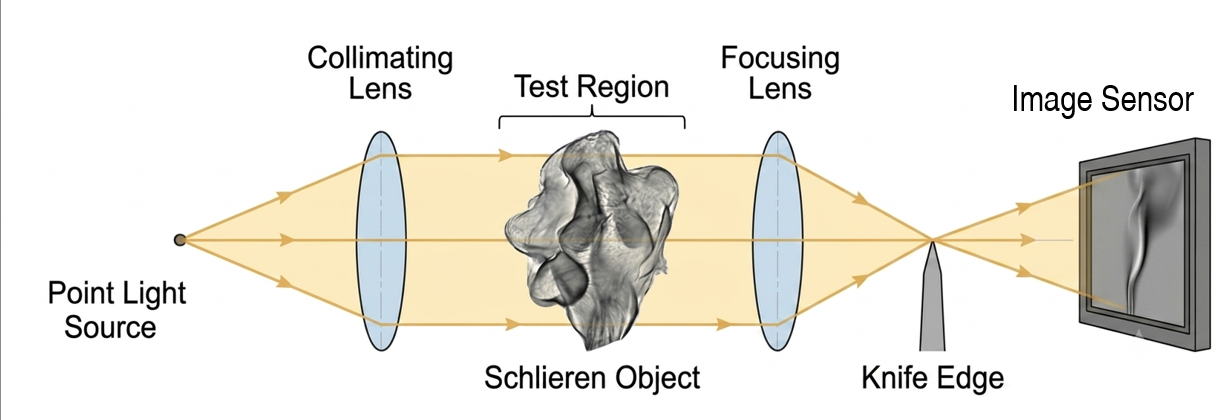
\includegraphics[trim={1cm 0cm 0cm 0cm}, clip, width=0.8\textwidth]{figures/Schlieren setup.png}
    \caption{Illustration of a simple schlieren setup}
    \label{fig: Schlieren setup}
\end{figure}


\par Another method that relies on light deviations to measure density gradients is interferometry. In this technique, the imaging sensor is exposed to two laser beams, one passes through the test subject, which bends it and slows it down; the other one reaches the sensor unaffected. When both beams interact with the imaging sensor, they interfere, producing interference fringes that can be related to the refractive index change in the test subject. One important application of the method is the use of laser speckle photography for interferometry by Debrus \cite{Debrus1972} and Köpf \cite{Kopf1972}. They used a ground glass lens diffuser to scatter the laser beam and produce a speckle pattern, then exposing a sensitive film to this laser-speckled pattern when there is an active flow and no flow passing through it. The double exposure produces Young’s fringes in the film which relates to light deviation \cite{NikitaFominBook}. Köpf’s setup can be seen in Figure \ref{fig: laser speckled interferometry}. This early use of speckle patterns foreshadows its later application in SBOS configurations.

\begin{figure}[htbp]
    \centering
    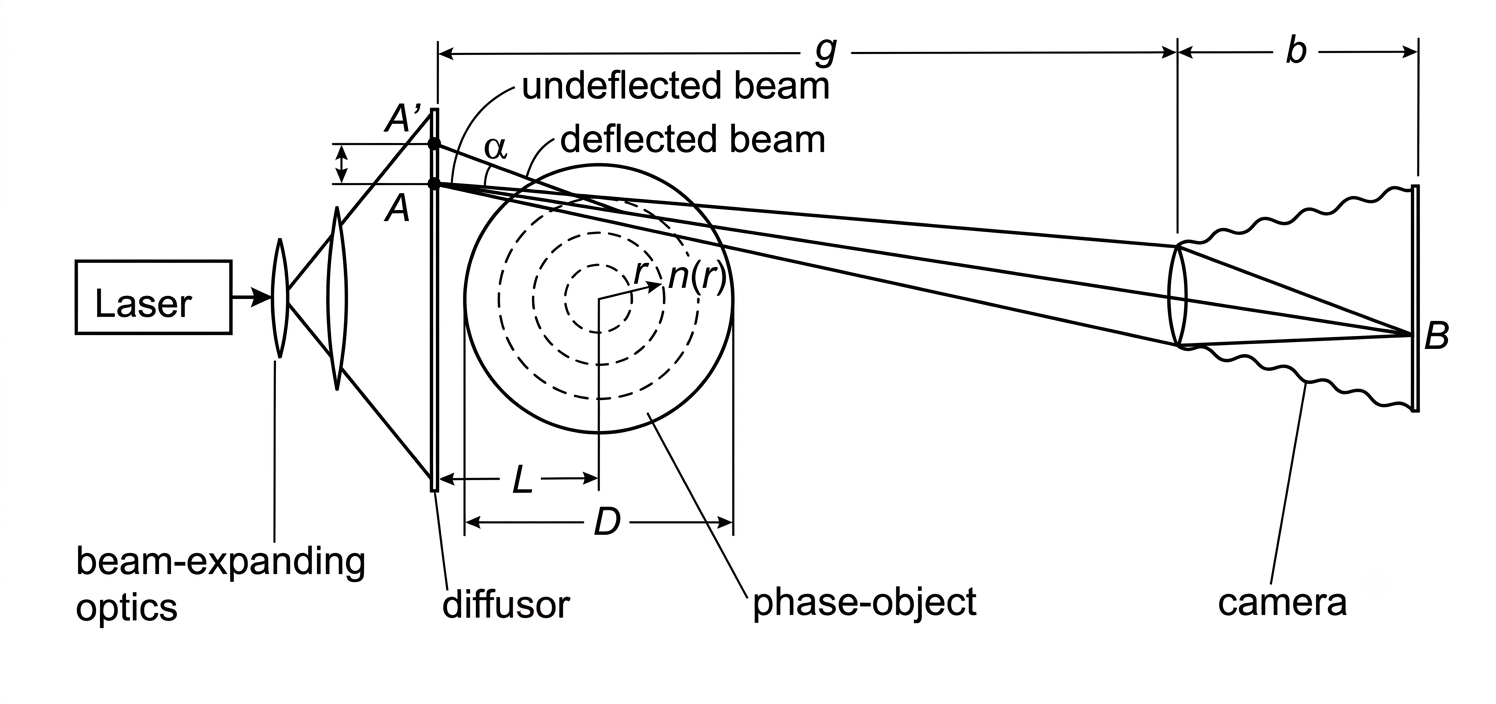
\includegraphics[width=0.8\textwidth]{figures/laser speckled interferometry.png}
    \caption{Laser-speckled Interferometry setup, credit to Köpf \cite{Kopf1972}}
    \label{fig: laser speckled interferometry}
\end{figure}

\par As aforementioned, the classical density gradient methods are still relevant to this day \cite{Settles2017}. Shadowgraphy’s simplicity gives relevant quick qualitative insights into the flow; Schlieren’s high sensitivity and small post-processing requirement motivates its use in many cases, with new developments even using colored filters to get information on more than one axis at a time; and Interferometry allowing for larger fields of view than the latter two. However, each of them lack in some way, as Shadowgraphy can only give qualitative results; Schlieren fails at larger scales and directional sensitivity; and interferometry uses a complicated setup with complex post-processing. Background Oriented Schlieren takes on the advantages of the latter methods and ameliorates its drawbacks, providing a simple, whole-field, scalable, high sensitivity technique, but still leaving some room for improvement, as will be discussed in the next section.

\section{Background Oriented Schlieren}
\label{section: Background Oriented Schlieren}
In the year 2000, a new technique emerged taking advantage of new sensors and image processing algorithms, the Background Oriented Schlieren (BOS) technique \cite{Raffel2001}. The method consists in measuring the distortion of a background image due to the presence of a test flow. To achieve that, a background pattern is positioned after the test section, an image of the pattern is captured when no flow is present and another when there is a density gradient that distorts the background. This displacement is quantified using image sensing algorithms and can be related to the flow’s density as shown in section \ref{section: Refraction} \cite{Schmidt2025}. This method greatly simplifies the Schlieren setup, provides a whole field analysis of the test section and it is easier to scale than the traditional methods. These advantages, together with its accuracy and non-intrusiveness, made the technique quite popular among experimentalists, with many improved versions being proposed over the years. Figure \ref{fig: BOS setup Raffel} shows a typical BOS setup.

\begin{figure}[htbp]
    \centering
    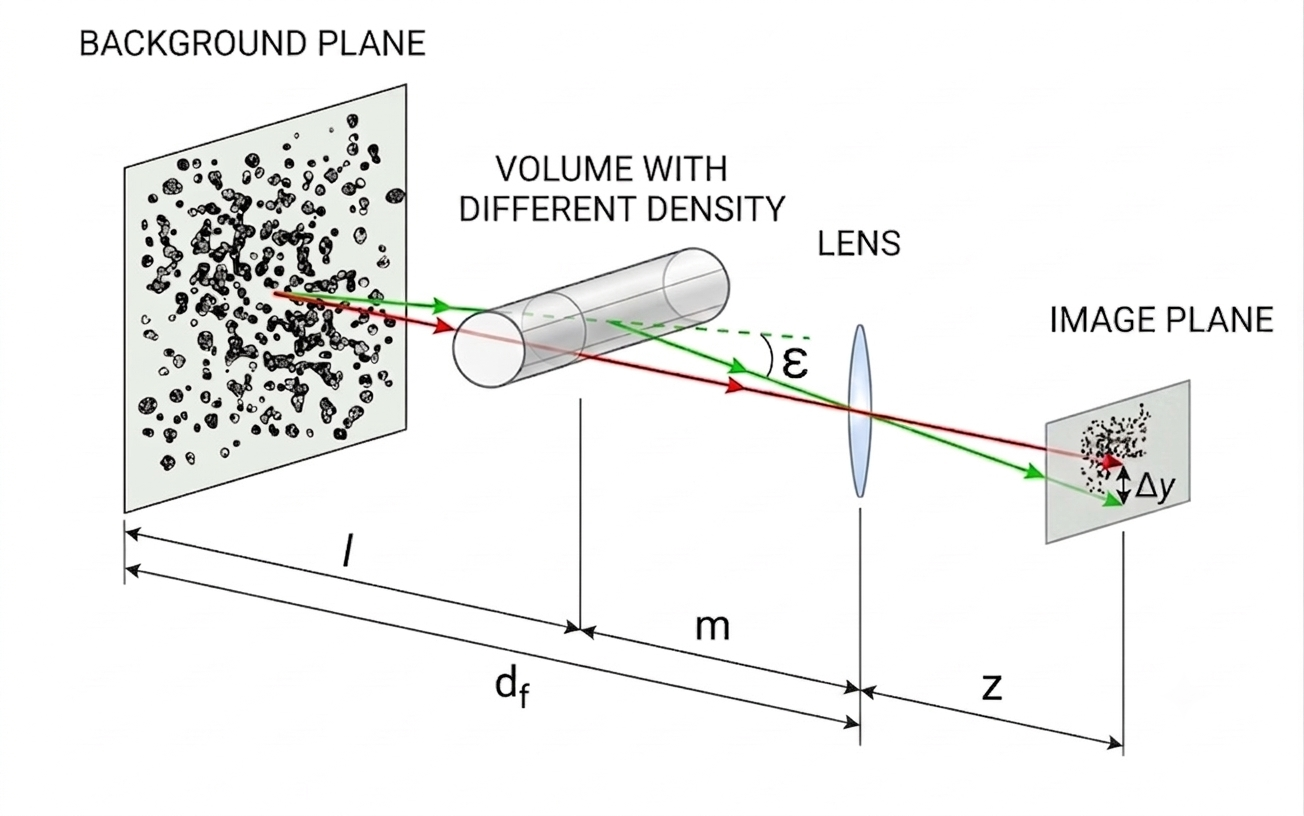
\includegraphics[width=0.6\textwidth]{figures/Raffel BOS setup.png}
    \caption{BOS setup, credit to Raffel \cite{Raffel2001}}
    \label{fig: BOS setup Raffel}
\end{figure}

%%% Now it comes the question. Should I talk about the equations now? Or leave then to mathodologies? a bit of both

\par Practical guidelines for the design of BOS setups have been established in the literature. Both Gojani et al. \cite{Gojani&Obayashi} and Schwarz et al.
\cite{Schwarz&Braukmann} highlighted the importance of sensitivity and spatial
resolution in defining the optical configuration for BOS. Sensitivity $S$ can be
interpreted as the capacity of the setup to magnify the light distortion from the
refractive object, and is set by the product of the defocus distance and the optical
magnification, $S = lM$. Spatial resolution refers to the smallest spatial scale of the studied flow that can be resolved, that is, the size of the smallest distinguishable flow feature $s_{min}$. It is governed by the blur of the refractive object, quantified by the circle of confusion $CoC$ \cite{Greenleaf1950}, its derivation can be found in Appendix \ref{Appendix: CoC derivation}. The complete set of relations linking these two performance parameters to the physical layout of the setup is assembled in Chapter \ref{chapter: methodology}, where it forms the basis of the design strategy of this thesis.

\par Sensitivity grows with the distance between the refractive object and the
background, so the first instinct is to place the background as far away as possible.
The returns diminish, however: as the defocus distance grows without bound the
sensitivity saturates at the focal length of the lens, $S \rightarrow f$. A longer
focal length therefore raises the ceiling on achievable sensitivity, but $f$ is itself
constrained by the desired field of view $L_{FoV_{obj}}$ and the camera sensor size
$L_{sens}$ \cite{Schmidt2025}. This asymptotic behavior is examined quantitatively in
Chapter \ref{chapter: methodology}.

\par Furthermore, there is an inherent focusing problem on BOS. During the setup assembly, one would like to focus on the background for better contrast and position the background farther away from the test subject for increased sensitivity. But, as the distance between the test subject and the in-focus plane increases, the blur of the refractive object is worsened and hinders the spatial resolution of the setup. One strategy would be to increase the depth of field, thus increasing the “thickness” of the in-focus plane, by increasing the $f_\#$ number (see Appendix~\ref{Appendix: CoC derivation} and \cite{Greenleaf1950}). However, reducing the lens aperture decreases the illumination reaching the camera sensor, which leads to reduced light signal and contrast. Consequently, a compromise must be made between spatial resolution and sensitivity, tuning the optical setup to achieve the maximum signal and acceptable blur.

\par Although it provides advantages compared to classical methods, the design of a BOS setup is marked by constraints and compromises. The achievable sensitivity is limited by the geometric configuration as increasing the sensitivity requires larger optical distances, which in turn degrade spatial resolution due to increased blur. Careful optimization of parameters is required to balance these competing effects. These limitations motivate the exploration of alternative approaches. By using Laser-Speckled Background Oriented Schlieren (SBOS) many of these shortcomings can be overcome, as it will be discussed. 

\par Before introducing SBOS, however, further aspects of BOS deserve attention. The first corresponds to an ambiguity found in the literature regarding the optical spatial resolution. Then, it will be discussed the influence of the imaging hardware and post-processing,as both bound accuracy and resolution as much as optics do. Lastly, a range of variants that has been derived from BOS over the past twenty-five years will be presented, which gives the context for understanding both the strengths and the particular niche SBOS occupies. The next subsections will treat these matters.
%I should maybe add a picture here

\subsection{Optical Spatial Resolution}
\label{subsection: Optical Spatial Resolution}
\par As  aforementioned, spatial resolution refers to the size of the smallest distinguishable feature in the image and in optical configurations that is limited by the amount of blur of the object. It is worth noting that, despite the clear conceptual definition, there is no consensus on a definitive mathematical formulation of this quantity in the literature, leading to ambiguity. Schwarz et al. \cite{Schwarz&Braukmann} tested various BOS setups and related the concept of Circle of Confusion ($CoC$) from Greenleaf \cite{Greenleaf1950} to the spatial resolution of the setup. Meanwhile, Gojani et al. \cite{Gojani&Obayashi} derived an equation for the spatial resolution using geometry and theoretical assumptions. The two formulations do not yield the same result, so an investigation on the methods used to obtain them was conducted.

\par Gojani et al.'s mathematical formulation has sound theoretical grounds, however it presents ambiguities and lack of experimental data to support some claims.  The paper makes the fundamental assumption that anything inside the $CoC$ is indistinguishable. Therefore, the smallest distinguishable size is obtained by tracing the cone of light from the $CoC$ in the sensor plane to a size in the object plane when the setup is focused on another plane (such as the background). Figure \ref{fig: Gojani cone of light} shows the cone of light used by Gojani to derive equation 10 in their article, showed in Appendix \ref{Appendix: Blurred Object} as equation \ref{equation: Gojani SR formulation}. On the image it is possible to see some distances that can be translated to the convention presented in Figure \ref{fig: BOS setup Raffel}, $s_t$ corresponds to the defocus distance $l$, $s_o$ is the in-focus distance $d_f$ and $s_i$ is the distance between the lens and the sensor $Z$.

\begin{figure}[h]
    \centering
    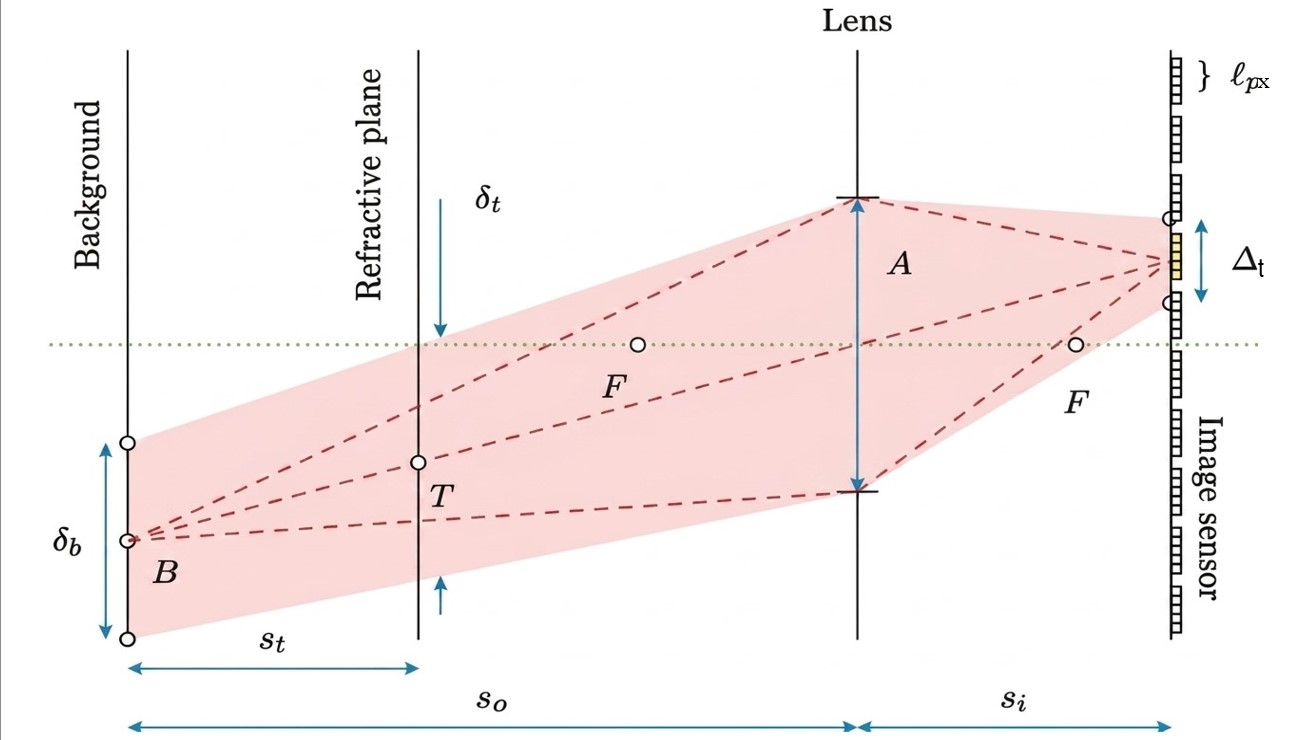
\includegraphics[width=0.8\textwidth]{figures/Gojani cone of light diagram.jpg}
    \caption{Diagram of the cone of light that reaches a length in the sensor $\Delta_t$, this image was used by Gojani et al. to derive his equation for spatial resolution. Credit to Gojani et al. \cite{Gojani&Obayashi}}
    \label{fig: Gojani cone of light}
\end{figure}

\par In Gojani's derivation of the blur circle $\delta_t$, they explicitly call the length in the sensor plane $\Delta_t$ as the "circle of confusion ($CoC$)" \cite{Gojani&Obayashi}. However, Ambiguity arises when they subsequently define it as a sampling cell $\Delta_t = k \cdot l_{px}$, where $k$ is a small integer and $l_{px}$ is the pixel pitch, do not explicitly say how $k$ is computed and fix $\Delta_t$ in the range of 5-50 $\mu$m. Appendix \ref{Appendix: Blurred Object} demonstrates that using Greenleaf's equation for the $CoC$ \cite{Greenleaf1950} to compute $\Delta_t$ places it outside that range for certain applications and yields a blur circle  $\delta_t = 2 \cdot CoC_{obj}$, which is four times the minimum distinguishable feature size $s_{min}$ measured by Schwarz and Braukmann \cite{Schwarz&Braukmann}. Moreover, no systematic experimental validation corroborating Gojani's claims has been found in the literature. Michalski used their formulation and attempted to compare it with the maximum density gradient width of a jet, still it was found to be only in a comparable order of magnitude to the computed value (width of 1.66 mm and $\delta_t$ of 0.86 mm) \cite{Michalski2018}. 

\par Contrasting to Gojani's approach, Schwarz and Braukmann systematically correlated $CoC$ with spatial resolution experimentally \cite{Schwarz&Braukmann}. First, they transferred the $CoC$ to refractive object plane by using a blurred object magnification, thus defining a $CoC_{obj}$ (this transfer was also derived in Appendix \ref{Appendix: Blurred Object}). Then, they obtained the smallest distinguishable size by measuring the contrast in light intensity of bright and dark bars of a resolution target for various optical setups. Schwarz's figure for spatial resolution is thus based on a separability criterion, it defines how close two points may lie before their image is merged. It was found that the minimum discernible feature was around half the $CoC_{obj}$, $s_{min} \approx 0.5 \cdot CoC_{obj}$. 

\par As it has been implicitly mentioned, Schwarz's result and Gojani's formulation are fundamentally different. Gojani derives the blur circle, whereas Schwarz is interested in a separability criterion. Therefore, Schwarz measure should be the radius of the circle derived by Gojani. Gojani's final formulation of $\delta_t$ in equation 12 corresponds to this, thus it is in agreement with Schwarz. However, his reasoning to drop the term containing $\Delta_t$ is weak, given that both terms in his formulation amount to the same value if $\Delta_t = CoC$, as shown by Appendix \ref{Appendix: Blurred Object}.

\par Ultimately, the experimental validation makes Schwarz's formulation the stronger of the two. Additionally, the loose definition of $\Delta_t$ in Gojani's formulation leads to ambiguity that can be interpreted into a result two times larger than the one corresponding to Schwarz's measurements. Since Schwarz's formulation is backed by experimental data, it is stronger than Gojani's and should be used to estimate the optical spatial resolution of a BOS setup. Therefore, the minimum distinguishable feature used for this thesis is the one derived by Schwarz and presented here in equation \ref{equation: smin}.

\par Up to this point, spatial resolution and sensitivity have been described primarily as functions of the optical setup, which governs the level of blur in the test section. However, these performance parameters are also significantly influenced by the choice of post-processing algorithms and hardware. Different image processing techniques can achieve varying levels of sensitivity and spatial resolution when converting captured images into displacement fields. While the characteristics of the background pattern such as speckle size and frequency also limits spatial resolution and influence the choice of post-processing algorithms. Therefore, each must be carefully selected for an experiment \cite{Schmidt2025}. 

\subsection{Imaging hardware and post-processing}
\label{subsection: Image processing}

%Add a picture on image processing?

\par On the imaging hardware level, the main parameter that influences resolution is the pixel density, which quantifies how many pixels correspond to a millimeter in the image. It is related to the magnification but also the size of the sensor and its pixels \cite{Schmidt2025, Gojani&Obayashi}. A smaller pixel size and higher magnification provides a higher pixel density, which means that a smaller feature can be imaged with more pixels, providing more detail. It is worth noting, that it is no use to have a higher spatial distribution of pixels if the blur limits the size of the smallest distinguishable feature. Consequently, an optimization must take place where the optical spatial resolution matches the hardware and post-processing resolution, so that the setup resources are used efficiently. Schwarz et al. make precisely this comparison by expressing both the circle of confusion and the interrogation window in the object domain and evaluating each against the size of the structure under study \cite{Schwarz&Braukmann}.

\par Once the BOS images are taken, they must be processed in a step that converts the recorded images into a displacement field data. The algorithm chosen for it bounds both the accuracy and the spatial resolution of the result. Cross-correlation (CC) was the first method applied to the technique \cite{Raffel2001} and remains the most widely used. Coming directly from its use in PIV, it divides the reference and the deflected image into interrogation windows, and uses a cross-correlation function applied to the intensity distribution of each window pair to find the displacement that best aligns them \cite{Schmidt2025}. One vector is returned per window, so the spacing of the resulting field follows from the window size $W$ and the fractional overlap $o$ as $W(1-o)$, for example, a 64 pixel window at $75\%$ overlap yields a vector every 16 pixels.

\par The inheritance from PIV comes with its drawbacks, Schmidt et al. \cite{Schmidt2025} point out two differences between the applications. Displacements in BOS are of the order of a few pixels rather than the ten to twenty typical of PIV \cite{Schmidt2025, Raffel2015}, so the dynamic range CC is designed to deliver goes largely unused while its penalty in accuracy and resolution is still present. Raffel notes that although displacements below half a pixel can still be determined with high accuracy, the smaller signal leaves BOS with relative errors of the order of 2--3\% of full scale against roughly 1\% for PIV \cite{Raffel2015}. Moreover, the background is manufactured in BOS as a field of discrete bright dots imitating tracer particles, which is not the best suited pattern to resolve a smooth displacement field \cite{Schmidt2025, CakirEtAl}.

\par These shortcomings motivated several alternatives. Iterative least squares (ILS) uses CC to locate the integer-pixel displacement and computes the subpixel part through a separate fit. This improves subpixel accuracy and reduces sensitivity to imaging noise. Optical flow (OF) abandons windows altogether and solves for the whole field at once, returning a vector at every pixel, at a computational cost roughly an order of magnitude above CC. Fourier demodulation (FCD) recovers the deflections from phase shifts in the Fourier domain and is faster than either, but demands a periodic background such as a sinusoid or a checkerboard. On idealized synthetic images OF and FCD reproduce the ground truth almost exactly, while CC and ILS visibly undersample sharp gradients \cite{Schmidt2025}, a ranking supported by Cakir et al. \cite{CakirEtAl}, who report a clear advantage of OF over CC in both accuracy and the range of resolvable density gradient amplitudes on a Prandtl-Meyer expansion fan.

\par Those margins narrow considerably in practice. Schmidt et al. observe that the advantage of a higher-fidelity algorithm is realized mainly when small-scale structures dominate and the images are essentially free of noise, and that defocusing can turn the advantages obsolete by blurring the fine scales out before processing begins \cite{Schmidt2025}. Schwarz et al. reach the same conclusion independently, reporting that in their own evaluations with synthetic BOS images they could not reliably match the resolution and accuracy of a $12 \times 12$ pixel cross-correlation using optical flow \cite{Schwarz&Braukmann}. Since a BOS setup is deliberately defocused on the refractive object, this technicality applies directly. Combined with the periodic pattern FCD demands, which a laser speckle field cannot provide, the computational cost of OF and the absence of both from commercially available packages, the practical balance favors cross-correlation with a potential iterative least squares refinement.

\par Within CC, the interrogation window governs the compromise between robustness and resolution. Indeed, Schwarz et al. name the window size and the geometric blur as the two factors that jointly limit the spatial resolution of a BOS measurement \cite{Schwarz&Braukmann}, so the optical and processing bounds cannot be chosen independently. Small windows are preferred in BOS precisely because the displacements are small \cite{Schmidt2025}, yet a window holding too few features yields an unreliable correlation peak. The minimum window size recommended in the literature ranges from four to five to ten background dots, depending on the author \cite{Schwarz&Braukmann}. Kähler et al. \cite{KahlerEtAl} quantified the resulting limit through the step response width, the smallest separation at which two vectors are genuinely independent, and showed it to grow both with the window size and the diameter of the imaged features. This means that a raise in the overlap produces a denser vector field without improving that independence, so the final window size, and not the vector spacing, is what sets the true spatial resolution of a measurement.

\par The same analysis determines the size of the background features themselves. Reliable subpixel interpolation of the correlation peak requires feature images larger than roughly two pixels. Below that threshold the fit can no longer locate the peak and the estimated displacements collapse toward integer values, an artifact known as peak locking \cite{KahlerEtAl}. Large features are equally unhelpful, since the step response width grows in proportion to their diameter, and once they reach about a quarter of the window size the partial features cut by the window edges degrade the response sharply. Holding the imaged feature between roughly two and five pixels satisfies both bounds. BOS literature converges on the same interval from experience: Raffel \cite{Raffel2015} reports background structures typically imaged at three to five pixels, with two to three preferable but rarely attainable because of diffraction at the small apertures BOS demands. He also cautions that the three-point peak fit inherited from PIV adds noise once the structures grow beyond that. Schwarz et al. quote an optimum dot image of about three pixels and worked at 3.4 to 5 pixels in their own experiments \cite{Schwarz&Braukmann}. For speckle backgrounds the same target applies, Michalski et al. sized their speckles at 61.6~\textmu m to cover roughly four pixels \cite{Michalski2018}. It is this requirement that is sought to be respected by the optical design of Chapter \ref{chapter: methodology}.

\par Processing and optics therefore impose complementary limits on what a BOS measurement can resolve. Neither has confined the technique to a single form: over the past twenty-five years it has been adapted to three-dimensional fields, to scales ranging from millimeters to aircraft in flight, and to backgrounds of very different kinds. Those developments are reviewed next.

\subsection{Variants of BOS}
\label{subsection: Variants of BOS}
\par Since BOS was introduced 25 years ago, the technique has not remained static, various authors have worked on modifications that enabled its application where it would be impractical to do so with the standard method. These developments were surveyed by Raffel \cite{Raffel2015} at the fifteen-year mark and, more recently, by Schmidt et al. \cite{Schmidt2025} across the full twenty-five years. A significant evolution was the development of tomographic BOS, which combines multiple camera perspectives to reconstruct three-dimensional density fields \cite{TomographicBOS, Raffel2015}. This method was demonstrated in applications ranging from supersonic wind tunnel tests to combustion imaging, and has since become the principal route to unsteady structures in variable-density flows \cite{Schmidt2025}. For setups where multiple cameras are unavailable, plenoptic BOS offers an alternative by capturing various perspectives from a single camera through a micro-lens array, enabling independent refocusing at different planes along the line of sight from a single image \cite{PlenopticBOS}. These modifications have greatly expanded the scope of BOS applications beyond single 2D gradient imaging.

%Add a picture here on one of these emethods

\par Other studies have focused on the limits of scaling BOS. At small scales, telecentric BOS addresses the geometric blur inherent to conventional setups through collection of parallel light rays onto the sensor \cite{TelecentricBOS}. This way perspective distortion is reduced and spatial resolution improved for fine-scale measurements. Van Hinsberg and Rösgen \cite{vanHinsberg2014} developed what they called Near-Field BOS. They modified the correction factor in the BOS relation presented by Dalziel et al. \cite{Dalziel2000} so that reliable densities can still be recovered when the background sits closely behind the flow. This removes the usual requirement for a large background-to-object distances. At larger scales, airborne BOS (AirBOS) has enabled schlieren imaging of supersonic aircraft in flight by using the Earth's natural surface texture as a background \cite{AirBOS, AirBOS2}, an approach whose viability rests on selecting terrain whose natural structures image at the same few-pixel scale demanded of a printed pattern \cite{Raffel2015, Schmidt2025}. Another method (BOSCO) has used celestial objects such as the Sun for the same purpose \cite{BOSCO}. Outdoor explosive and ballistic tests have  also leveraged natural backgrounds and zebra board patterns to visualize shock wave propagation over fields of view inaccessible to laboratory optics \cite{ExplosionsBOS, Schmidt2025}. As a result, BOS can be applied in contexts where normal schlieren would have been impractical as it would need unreasonably heavy and large optical elements.

\par For high-speed applications that demand high luminous intensity, developments have been made in background illumination strategies. Back-illuminated transparent patterns and retroreflective sheeting with co-linear illumination have both been demonstrated as effective solutions in large-scale ground test facilities \cite{RBOS, BackIluminatedBOS}. As Raffel \cite{Raffel2015} mentions, the methods are motivated by the fact that a small aperture is wanted to limit blur but starves the sensor of light, while short exposures are wanted to limit motion blur. Therefore, retroreflective material is valuable precisely because its on-axis return does not obey the inverse-square law that penalizes a diffuse background, allowing for better contrast. The same design pressure has driven sensor technology, from pulsed and high-framing-rate BOS \cite{Raffel2015} to event-based cameras, which record only pixel-level brightness changes, allowing them to reach kHz rates at a fraction of the illumination power and cost \cite{Schmidt2025}. More recently, laser speckle has been proposed as a background source due to its high intensity and the always-in-focus nature of the speckle pattern at the sensor \cite{Meier&Roesgen2013}, properties that form the conceptual basis for the SBOS method investigated in this thesis.

\section{Laser Speckled Background Oriented Schlieren}
\label{sectio: Laser Speckled BOS}
\par Laser-Speckled Background Oriented Schlieren is based on the same principles of BOS, with the distinct difference that a laser speckled pattern is used as reference instead of a physical background pattern. The speckle pattern is a result of the constructive and destructive interference caused by the interaction of scattered wavefronts originating from a previously collimated coherent light source, which arrive at the sensor with random phase differences. This interference pattern has been extensively investigated since the 1960s \cite{NikitaFominBook, Goodman2020} and has found applications in diversified fields such as the imaging of blood flow in medical fields \cite{Boas&Dunn2010}, non destructive analysis of structural materials through shearography \cite{Hung&Ho2005} and the study of density gradients using laser speckled interferometry \cite{Debrus1972}. However, the first reported use of a laser speckle pattern as a BOS background was by Meier and Rösgen in 2013 \cite{Meier&Roesgen2013}. It can be said then that SBOS is a relatively new development and being this recent, it is yet to be largely applied and studied, presenting the opportunity for novel and interesting developments.

\par Speckle creation has been extensively treated by Goodman \cite{Goodman2020} and its application to fluid mechanics measurements by Fomin \cite{NikitaFominBook}. As aforementioned, the speckles are created when light gets scattered by a surface rougher than its wavelength, which randomly changes the amplitude and the optical path length of the scattered rays and thus creates an interference pattern. This surface can be a rough projection plane or a diffuser such as a ground glass. The speckles can either be objective, when the scattered light propagates freely to an observation plane; or subjective, when it is collected by a lens. It is worth highlighting that speckle creation is random at its core \cite{Cloud2007, Goodman2020}. As a consequence, the theoretical mathematical treatment of this phenomenon involves complex Fourier analysis and statistics, which were considered out of scope. This thesis will treat more on the practical aspects of speckle generation and try to develop practical guidelines for its use.

\par The work of Meier and Rösgen \cite{Meier&Roesgen2013} introduced SBOS and showed that using a laser speckled background greatly expands the design space of a BOS experimental setup. By creating subjective speckles, the exit pupil of the imaging system itself can be regarded as the effective scattering spot \cite{Goodman2020}. Consequently, the speckles stay sharp at any virtual position the camera has its focus on. This permits the positioning of the pattern to be virtually anywhere along the laser beam, be it in front of the refractive object, inside of it, behind it, or even beyond the scattering plane. Consequently, optical arrangements that would be impossible in conventional BOS become feasible with SBOS. A picture of their experimental setup can be seen in Figure \ref{fig: SBOS Meier and Roesgen}.

\begin{figure}[h]
    \centering
    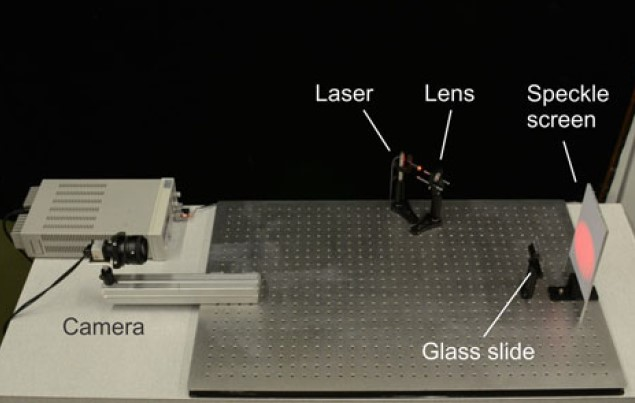
\includegraphics[width=0.6\textwidth]{figures/Meier and Roesgen single pass setup.jpg}
    \caption{Experimental SBOS setup (single pass) used by Meier and Rösgen \cite{Meier&Roesgen2013}}
    \label{fig: SBOS Meier and Roesgen}
\end{figure}

\par These new optical configurations promise great benefits compared to standard BOS \cite{Meier&Roesgen2013}. By focusing the camera in front of the test section, a larger increase in sensitivity can be achieved while maintaining the same spatial resolution. Positioning the focus beyond the physical position of the screen allows for larger effective defocusing distances while maintaining the screen close to the test section, which greatly reduces the physical size of the setup. Focusing the camera inside the test section improves the spatial resolution; the implications for image quality and sensitivity, however, are not clear. Meier and Rösgen also developed the double-pass mode, where the laser beam is directed coaxially with the camera through the test section, effectively doubling the sensitivity by capturing the deflection of both the illumination beam and the imaging path. The ability to choose among these optical configurations alleviates the constraints between sensitivity and spatial resolution present in standard BOS, allowing for a much more optimized optical setup. 

\par Furthermore, replacing the conventional printed background with a laser-generated speckle pattern offers advantages in terms of background quality and spatial frequency content. Unlike physical background patterns, whose feature size is constrained by printing and manufacturing limitations, the minimum speckle diameter is only limited by the Rayleigh diffraction criterion \cite{Barker&Fourney}. If the interference pattern becomes diffraction limited due to the camera aperture, it will be only constrained by the laser wavelength, the f-stop number and the camera magnification. Consequently, SBOS can produce significantly finer background structures, providing higher spatial-frequency information for image correlation and potentially improving the spatial resolution.

\par After the work of Meier and Rösgen, only a limited number of studies have explored SBOS experimentally. Bühlmann \cite{Buhlmann2020} employed the technique in the tomographic imaging of a heated jet near a wall where the laser-speckle was projected as a background. His measurements highlight the potential of SBOS as they would have been unfeasible with conventional BOS. Michalski et al. \cite{Michalski2018} applied the method using the in-focus plane in front of the refractive object to obtain the calorimetry of an electrical spark discharge. In contrast to the previously mentioned works that used a scattering screen, Michalski et al. used a ground glass diffuser to scatter the laser beam and pointed it directly to the camera sensor, much similar to the setup used by Debrus on speckle interferometry \cite{Debrus1972} as it can be seen in Figure \ref{fig: SBOS setup illustrated}. Their work also rigorously quantified the method's uncertainties and compared its accuracy with standard BOS, which will be discussed in the next section. Nakamura et al. \cite{Nakamura2021} also employed laser speckles in a different way to develop a methodology intended to compute the depth location of refractive structures inside the test section and used a compressible jet to demonstrate it. Both Nakamura's and Michalski's work highlight the usefulness of SBOS for imaging fast phenomena with low signal-to-noise ratio. These studies demonstrate the method's potential, nevertheless, most of its developments have originated from a small number of research groups. Consequently, important questions regarding implementation, uncertainty, spatial resolution, and applicability in demanding environments remain insufficiently explored.

\begin{figure}[htbp]
    \centering
    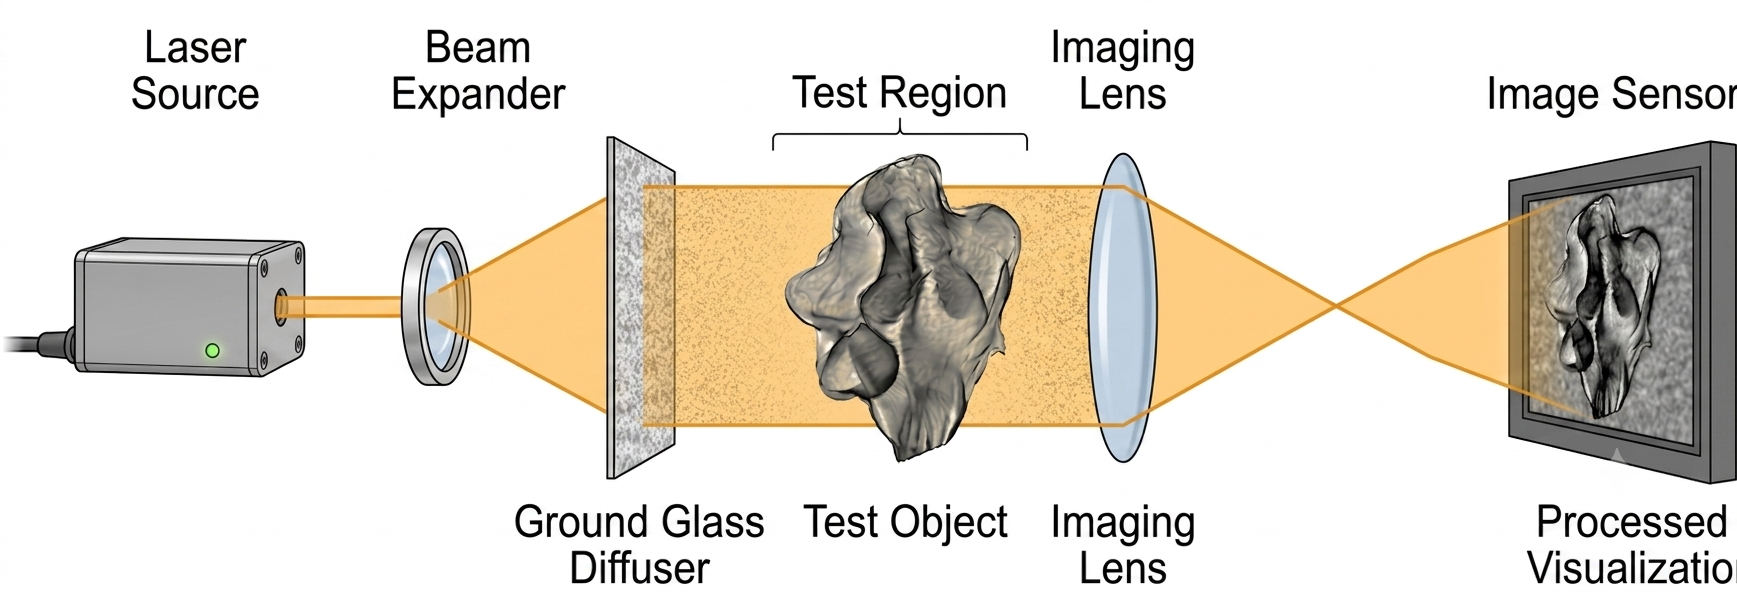
\includegraphics[width=0.6\textwidth]{figures/SBOS setup ilustrated.png}
    \caption{Illustration of a SBOS setup using ground-glass-diffused laser speckles, similar to Michalski's setup \cite{Michalski2018}}
    \label{fig: SBOS setup illustrated}
\end{figure}

\subsection{Limitations, accuracy and uncertainty of SBOS}

\par Despite its advantages, SBOS presents some constraints and drawbacks that must be considered in its implementation. Some of these are shared with BOS such as spatial resolution and sensitivity constraints due to the chosen processing algorithms and hardware. Others are exclusive to SBOS, such as higher complexity and possible decorrelation problems. This subsection will discuss how literature treats these limitations and how it provides a comparison of the method’s accuracies and uncertainties with standard BOS.

\par A natural complication of SBOS is the increased complexity that comes with using a laser instead of a physical background. It requires laser compatible lenses, more optical elements, special care when handling and maintaining the setup and additional safety concerns as the laser presents a hazard at high energy settings. By implementing the method, a trade-off must be made between the increased complication and the gains in resolution and sensitivity; this will be treated in more depth in the methodology chapter.

\par It is also worth noting that there have been two ways in the literature to generate the speckle pattern and both have been used successfully for SBOS. It is possible to classify them into projected speckles employed by Bühlmann \cite{Buhlmann2020} and Meier and Rösgen \cite{Meier&Roesgen2013}, and directed speckles used by Michalski et al. \cite{Michalski2018} and Nakamura et al. \cite{Nakamura2021}. It is not clear which one of them is more effective in generating speckles, that is, what the drawbacks and advantages of each approach are. It might be only a matter of convenience when only one optical access is available, maybe one of the methods presents a more uniform distribution of speckles or is more prone to decorrelation than the other. Given the lack of literature on the topic, it would be interesting to test them both and compare them.

\par Decorrelation is the failure to correlate the background shift with the reference pattern and it's a phenomenon that might arise when using a laser speckled pattern as background. Bühlmann encountered this as a substantial problem on his projected laser speckle setup, which required him to use large cross-correlation windows and apply corrections for the pattern shift \cite{Buhlmann2020}. Li and Chiang have researched decorrelation effects for laser speckle interferometry and concluded that the main sources of the effect are surface tilt, out-of-plane displacement and lens aberration \cite{Li&CHiang1986}. Meier and Rösgen have also mentioned linear induced errors due to projecting surface tilt, so it could be that using projected speckles, like in Bühlmann’s setup, makes the method more prone to decorrelation \cite{Meier&Roesgen2013}. Neither Nakamura et al. nor Michalski et al. have reported the issue in their direct laser-speckle setups, which suggests that the effect could be mitigated by this approach \cite{Nakamura2021, Michalski2018}.

\par Regarding the accuracy of the technique, both Michalski and Nakamura quantified errors in their applications \cite{Michalski2018, Nakamura2021}. Michalski et al. validated their implementation with a CO$_2$  jet and obtained a mean density for the core $0.8\% \pm 0.9\%$ lower than expected, yielding a $0.3\% \pm 0.3\%$ error for the final measured CO$_2$ density. Nakamura et al. described an approximated error of $10\%$ on their method to identify the depth position of refractive objects, but did not show the errors of their density field. Compared to BOS, whose measurement error has been found to be in the order of $2-3\%$ of the full scale by Raffel\cite{Raffel2015} and Elsinga et al. \cite{Elsinga2004} reporting an accuracy of around $2\%$ against theory for a Prandtl--Meyer expansion fan, SBOS applied by Michalski et al. performs well in terms of accuracy.

\par Uncertainty and noise are also important aspects to ascertain in experimental techniques. Michalski et al. \cite{Michalski2018} and Meier and Rösgen \cite{Meier&Roesgen2013} mention that the increased sensitivity of SBOS also makes it more prone to noise from vibration coming from setup equipment. Moreover, noise could come intrinsically from the camera sensor, room temperature gradients and even the image processing algorithm. Michalski et al. estimated the total uncertainty in their setup, quantifying partial uncertainties from the integration method, magnification, defocusing distance, cross-correlation, tomographic reconstruction and white noise, reaching a final value of $6.2\%$. In this project, the uncertainty sources of the designed setup will be documented in Chapter \ref{chapter: Experimental Setups} and their impact quantified in the results.

\section{Research Gap}

\par The literature review reveals that SBOS is a promising, but not yet mature, technique. While Meier and Rösgen established its conceptual foundation and demonstrated its advantages over standard BOS \cite{Meier&Roesgen2013}, the subsequent body of work remains sparse, originating largely from a small number of research groups and covering a narrow range of applications. This contrasts sharply with the extensive and well-validated literature surrounding conventional BOS. Three clusters of open questions emerge from this review. First, no systematic implementation guidelines exist for SBOS setup design. The sensitivity-resolution trade-off is well characterized for BOS, but whether and how those relationships translate to SBOS configurations, particularly for unusual background placements, has not been thoroughly addressed. Second, uncertainty quantification remains incomplete. Michalski et al. provide the most rigorous treatment to date \cite{Michalski2018}, but their setup is specific enough that their uncertainty budget cannot be straightforwardly transferred to other configurations. Third, the behavior of SBOS in demanding high-speed wind tunnel environments is entirely unexplored, leaving open questions about decorrelation, vibration sensitivity, and optical feasibility under those conditions.

\par Together, these gaps mean that a researcher wishing to implement SBOS today would find no coherent roadmap to follow. The present thesis addresses this by designing, building, and systematically investigating an SBOS setup, using a high-speed wind tunnel application as the target demonstration case. The specific research questions motivating this work are stated in Chapter \ref{chapter: introduction}.